\section[Свойства многочленов Чебышёва первого рода: симметричность, нули, экстремумы.]{Свойства многочленов Чебышёва первого
  рода: \\ симметричность, нули, экстремумы.}

\begin{definition}
  Многочленами Чебышёва первого рода называется последовательность
  многочленов, удовлетворяющих рекурентному соотношению
  \[T_{n+1}(x)=2xT_n(x)-T_{n-1}(x),\ T_0(x)=1,\ T_1(x)=x\]
\end{definition}

\begin{theorem}
  Старший коэффициент многочленов Чебышёва имеет вид $T_n(x)=2^{n-1}x^n+\ldots$
\end{theorem}

\begin{proof}
  База индукции $T_2=2x^2-1$ - верна. Шаг индукции:
  \[T_{n-1}(x)=2^{n-2}x^{n-1}+\ldots\Rightarrow T_n(x)=2xT_n(x)+T_{n-1}(x)=2x\cdot(2^{n-2}x^{n-1}+\ldots)+\ldots=2^{n-1}x^n+\ldots\]
\end{proof}

\begin{theorem}
  \[T_{2n}(-x)=T_{2n}(x),\ T_{2n+1}(-x)=-T_{2n+1}(x)\]
\end{theorem}

\begin{proof}
  По индукции.
\end{proof}

\begin{theorem}
  Два различных многочлена Чебышёва ортогональны относительно
  скалярного произведения $(T_n,T_m)_{p(x)}$, где вес $p(x)=\frac{1}{\sqrt{1-x^2}} > 0$ п.в.
  \[\int_{-1}^{1}\frac{T_n(x)T_m(x)}{\sqrt{1-x^2}}dx=\begin{cases}
      0,\ m\neq n\neq0         \\
      \frac{\pi}{2},\ m=n\neq0 \\
      \pi,\ m=n=0              \\
    \end{cases}\]
\end{theorem}

\begin{proof}
  Переходим к тригонометрической форме
  \begin{multline*}
    \int_{-1}^{1}\frac{\cos(n\arccos(x))\cos(m\arccos(x))}{\sqrt{1-x^2}}dx
    =\Big|\substack{x=\cos\varphi \\
      dx = -\sin\varphi d\varphi\\
      1\rightarrow0 \\
      -1\rightarrow\pi
    }\Big|=\int_{0}^{\pi}\frac{\cos(n\varphi)\cos(m\varphi)}{\sin\varphi}\sin\varphi d\varphi = \\
    = \frac{1}{2}\int_0^{\pi}\cos((n+m)\varphi)+\cos((n-m)\varphi)d\varphi = \frac{\sin((n+m)\varphi)}{2(n+m)}\Big|_0^{\pi}+\frac{\sin((n-m)\varphi)}{2(n-m)}\Big|_0^{\pi}=\begin{cases}
      0,\ m\neq n\neq0         \\
      \frac{\pi}{2},\ m=n\neq0 \\
      \pi,\ m=n=0              \\
    \end{cases}
  \end{multline*}
\end{proof}

\tikzset{
  trig_circle/.pic={
      code={
          \coordinate (O) at (0,0);
          \draw[thick,->] (0,-1.5) -- (0,1.5);
          \draw[thick,->] (-1.5,0) -- (1.5,0);
          \draw (O) circle (1);
        }}
}

\def\SingleImageScale {1.3}

\begin{theorem}
  $T_n(x)$ на отрезке $[-1,1]$ имеет $n$ различных корней $x_m=\cos\frac{(2m-1)\pi}{n}$.
\end{theorem}

\begin{proof} Найдем корни уравнения тригонометрической формы.
  \[\cos(n\arccos(x_m))=0 \Leftrightarrow n\arccos(x_m)=-\frac{\pi}{2}+\pi m,\ m=0,\pm1,\pm2,\ldots\]
  \[x_m=\cos\left(\frac{\pi(2m-1)}{2n}\right),\ m=0,\pm1,\pm2,\ldots\]
  Получили много корней, а в теореме всего $n$. Посмотрим внимательнее на корни.

  \begin{figure}[h]
    \centering
    \begin{minipage}{.5\linewidth}
      \centering
      \tikzsetnextfilename{07/OddRoots}
      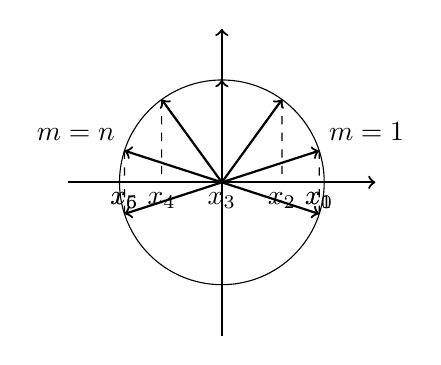
\begin{tikzpicture}[scale=\SingleImageScale]
        \path (0,0) pic[transform shape] {trig_circle};
        \def\n {5};
        \foreach \m in {0,1,...,6} {
            \def\ang {deg((2*\m-1)*pi/(2*\n))};
            \draw[thick,->] (O) -- ({cos(\ang)},{sin(\ang))}) coordinate (c_\m);
            \draw[dashed] (c_\m) -- ({cos(\ang)},0) node[below]{$x_{\m}$};
          }
        \node [anchor=south west] at (c_1){$m=1$};
        \node [anchor=south east] at (c_\n){$m=n$};
      \end{tikzpicture}
    \end{minipage}\hfill
    \begin{minipage}{.5\linewidth}
      \centering
      \tikzsetnextfilename{07/EvenRoots}
      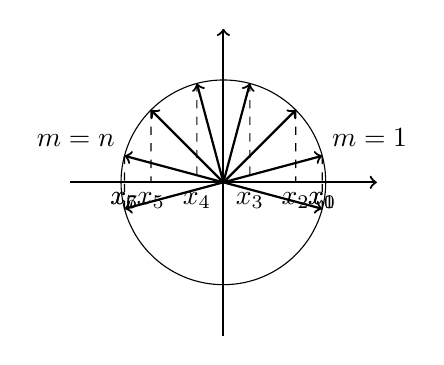
\begin{tikzpicture}[scale=\SingleImageScale]
        \path (0,0) pic[transform shape] {trig_circle};
        \def\n {6};
        \foreach \m in {0,1,...,7} {
            \def\ang {deg((2*\m-1)*pi/(2*\n))};
            \draw[thick,->] (O) -- ({cos(\ang)},{sin(\ang))}) coordinate (c_\m);
            \draw[dashed] (c_\m) -- ({cos(\ang)},0) node[below]{$x_{\m}$};
          }
        \node [anchor=south west] at (c_1){$m=1$};
        \node [anchor=south east] at (c_\n){$m=n$};
      \end{tikzpicture}
    \end{minipage}
    \caption[odd]{Корни при $n=5$ и $n=6$}
  \end{figure}

  Из полученных множеств нужно выбрать только различные, а их как раз $n$.
  Обратим так же внимание, что при представлении в тригонометрической
  форме мы заложились, что $|x|\leq1$, но так как на $[-1,1]$ мы нашли все $n$
  корней, а у полинома $n$-ой степени больше быть не может, то мы нашли корни $\forall\ x\in \R$
\end{proof}

\begin{theorem}
  На отрезке $[-1,1]$ имеется $n+1$ экстремум, $T_n(x_{(m)})=(-1)^m$. Экстремумы имеют вид
  \[x_{(m)}=\cos\frac{\pi m}{n},\ m=0,\ldots,n\]
\end{theorem}

\begin{proof}
  Найдем экрстремумы уравнения тригонометрической формы.
  \[\cos(n\arccos(x_{(m)})=\pm1 \Leftrightarrow n\arccos(x_{(m)})=\pi m,\ m=0,\pm1,\pm2,\ldots\]
  \[x_{(m)}=\cos\frac{\pi m}{n},\ m=0,\pm1,\pm2,\ldots\]
  Ищем различные экстремумы, аналогично корням, получаем $n+1$ штуку.
  \begin{figure}[h]
    \centering
    \begin{minipage}{.5\linewidth}
      \centering
      \tikzsetnextfilename{07/OddExtr}
      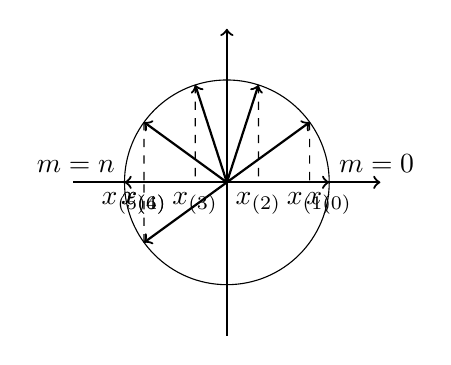
\begin{tikzpicture}[scale=\SingleImageScale]
        \path (0,0) pic[transform shape] {trig_circle};
        \def\n {5};
        \foreach \m in {0,1,...,6} {
            \def\ang {deg(\m*pi/(\n))};
            \draw[thick,->] (O) -- ({cos(\ang)},{sin(\ang))}) coordinate (c_\m);
            \draw[dashed] (c_\m) -- ({cos(\ang)},0) node[below]{$x_{(\m)}$};
          }
        \node [anchor=south west] at (c_0){$m=0$};
        \node [anchor=south east] at (c_\n){$m=n$};
      \end{tikzpicture}
    \end{minipage}\hfill
    \begin{minipage}{.5\linewidth}
      \centering
      \tikzsetnextfilename{07/EvenExtr}
      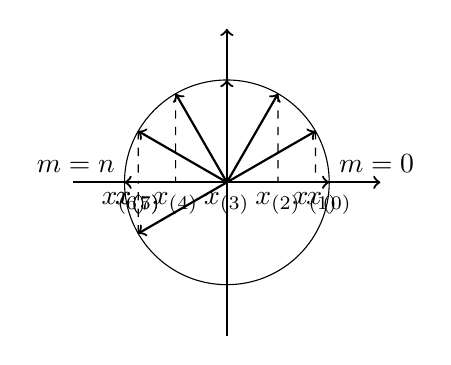
\begin{tikzpicture}[scale=\SingleImageScale]
        \path (0,0) pic[transform shape] {trig_circle};
        \def\n {6};
        \foreach \m in {0,1,...,7} {
            \def\ang {deg(\m*pi/(\n))};
            \draw[thick,->] (O) -- ({cos(\ang)},{sin(\ang))}) coordinate (c_\m);
            \draw[dashed] (c_\m) -- ({cos(\ang)},0) node[below]{$x_{(\m)}$};
          }
        \node [anchor=south west] at (c_0){$m=0$};
        \node [anchor=south east] at (c_\n){$m=n$};
      \end{tikzpicture}
    \end{minipage}
    \caption[odd]{Экстремумы при $n=5$ и $n=6$}
  \end{figure}
\end{proof}

Таким образом, мы можем сделать вывод о том как выглядят
многочлены Чебышева.
\begin{figure}[h]
  \centering
  \begin{minipage}{.5\linewidth}
    \centering
    \tikzsetnextfilename{07/OddCheb}
    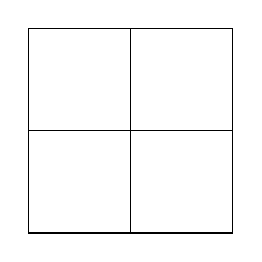
\begin{tikzpicture}[scale=\SingleImageScale]
      \def\n {5};
      \draw (-1,-1) grid (1,1);
      \draw[domain=-1:1,samples=100] plot[id=cheb] function{cos(\n * acos(x))};
    \end{tikzpicture}
  \end{minipage}\hfill
  \begin{minipage}{.5\linewidth}
    \centering
    \tikzsetnextfilename{07/EvenCheb}
    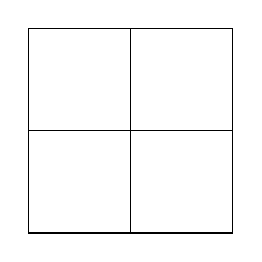
\begin{tikzpicture}[scale=\SingleImageScale]
      \def\n {6};
      \draw (-1,-1) grid (1,1);
      \draw[domain=-1:1,samples=100] plot[id=cheb] function{cos(\n * acos(x))};
    \end{tikzpicture}
  \end{minipage}
  \caption[odd]{Многочлены Чебышёва степени $n=5$ и $n=6$}
\end{figure}

% Теоремы о композиции.
% Не вошли в программу.
